% =========================================================================
%  Early Detection of Overfitting via Persistent Homology Analysis
%  of Deep Neural Network Activations
% =========================================================================
\documentclass[11pt,a4paper]{article}

% --- Encoding and language ---
\usepackage{fontspec}
\usepackage{polyglossia}
\setmainlanguage{english}

% --- Mathematics ---
\usepackage{amsmath,amssymb,amsthm}
\usepackage{mathtools}

% --- Figures and tables ---
\usepackage{graphicx}
\usepackage{float}
\usepackage{booktabs}
\usepackage{subcaption}
\usepackage[justification=centering]{caption}

% --- Page layout ---
\usepackage[margin=2.5cm]{geometry}
\usepackage{setspace}
\onehalfspacing
\usepackage{parskip}

% --- Colors ---
\usepackage{xcolor}

% --- Hyperlinks and references ---
\usepackage[backend=biber, style=numeric, sorting=none, doi=true, url=true, eprint=true]{biblatex}
\addbibresource{references.bib}
\usepackage[hidelinks]{hyperref}
\usepackage{cleveref}

% --- Algorithms ---
\usepackage[ruled,vlined]{algorithm2e}
\crefname{algocf}{algorithm}{algorithms}
\Crefname{algocf}{Algorithm}{Algorithms}

% --- Theorem environments ---
\newtheorem{definition}{Definition}[section]
\newtheorem{proposition}{Proposition}[section]
\newtheorem{remark}{Remark}[section]

% --- Custom commands ---
\newcommand{\R}{\mathbb{R}}
\newcommand{\N}{\mathbb{N}}
\newcommand{\Hk}{H_k}
\newcommand{\betti}{\beta}
\newcommand{\VR}{\mathrm{VR}}
\newcommand{\PE}{\mathrm{PE}}
\newcommand{\Dgm}{\mathrm{Dgm}}
\newcommand{\moy}[1]{\overline{#1}}
\newcommand{\ecart}{\pm}

% =========================================================================
\title{%
  \textbf{Early Detection of Overfitting via Persistent Homology Analysis
  of Deep Neural Network Activations}
}

\author{%
  Denis Chaput\\
  {\small Independent Researcher --- Topological Data Analysis}
}

\date{February 2026}

% =========================================================================
\begin{document}
\maketitle

% =========================================================================
\begin{abstract}
Overfitting constitutes a fundamental challenge in deep learning.
Classical detection methods rely on monitoring validation loss, often
a lagging indicator. In this work, we propose an approach based on
Topological Data Analysis (TDA) to detect early signs of
overfitting. We compute the persistent homology of internal activations
of neural networks trained under controlled overfitting conditions. Our
study covers three datasets (Fashion-MNIST, CIFAR-10, MNIST), three
architectures (shallow CNN, deep CNN, MLP), and four training set sizes,
following a one-factor-at-a-time design (8 configurations total),
with five independent runs per configuration to ensure statistical
reproducibility. The topological invariants---in particular the smoothed
derivative of $\PE(H_1)$ and $\betti_1$---are quantitatively compared
to four classical detectors (early stopping, loss gap, gradient norm,
weight norm). Our results show that detection based on the derivative
of $\PE(H_1)$ triggers on average at epoch $23.6 \ecart 6.1$ on
Fashion-MNIST/CNN, compared to $77.0$ for early stopping (patience${}=10$),
while maintaining a $100\%$ detection rate across all tested configurations.
The stability of topological invariants with respect to subsampling is
validated through bootstrap analysis.
\end{abstract}

Keywords: Topological data analysis, persistent homology,
overfitting, deep neural networks, persistent entropy, Betti numbers,
change-point detection.

% =========================================================================
\section{Introduction}
\label{sec:introduction}

Deep learning has revolutionized numerous fields, from computer vision
to natural language processing. However, a recurrent problem persists:
overfitting, where the model memorizes training data at the
expense of its generalization capacity~\cite{naitzat2020topologydeepneuralnetworks}.

Classical methods for detecting overfitting primarily rely on monitoring
validation loss (early stopping) or indirect indicators such as weight
norms, gradient norms, or measures of loss surface ``flatness''
\cite{foret2021sharpnessawareminimizationefficientlyimproving}. These approaches have limitations:
early stopping is a lagging indicator that only signals degradation after
it has set in; weight and gradient norms are indirect proxies that do not
characterize the geometry of internal representations.

Topological Data Analysis (TDA) offers a rigorous mathematical framework
for characterizing the ``shape'' of data across scales
\cite{Carlsson2009TopologyAD, chazal2021introductiontopologicaldataanalysis}. In particular,
persistent homology enables the detection of topological structures
(connected components, loops, cavities) and tracks their evolution
throughout a filtration~\cite{Edelsbrunner2002, Ghrist2007BarcodesTP}.
Recent work has shown that the topology of internal representations in
a neural network evolves during training
\cite{naitzat2020topologydeepneuralnetworks, rieck2019neural, guss2018characterizingcapacityneuralnetworks}.
Naitzat et al.~\cite{naitzat2020topologydeepneuralnetworks} demonstrated that successive
layers of a deep network progressively simplify data topology. Rieck
et al.~\cite{rieck2019neural} proposed neural persistence as a
complexity measure. Corneanu et al.~\cite{corneanu2020computingtestingerrortesting} explored
the links between decision boundary topology and generalization error.

Building on these observations, an important question is whether the evolution of internal representation topology can serve as an early indicator of overfitting, and how it compares to classical detection methods.

\paragraph{Contributions.} Based on these questions, this work provides the following contributions:
\begin{enumerate}
  \item A systematic study of topological evolution of activations under
  controlled overfitting, covering 3 datasets, 3 architectures,
  and 4 training set sizes in a one-factor-at-a-time design
  (8 configurations total).

  \item A quantitative comparison between topological detectors
  (CUSUM and smoothed derivative on $\PE(H_1)$ and $\betti_1$) and four
  classical detectors (early stopping, loss gap, gradient norm, weight norm),
  with 5 independent runs per configuration.

  \item A stability analysis via bootstrap of topological invariants
  with respect to subsampling.

  \item The identification of a three-phase pattern (compression, stabilization,
  fragmentation), where the third phase constitutes a potential precursor
  signal of overfitting.
\end{enumerate}

% =========================================================================
\section{Mathematical Foundations}
\label{sec:background}

We briefly recall the essential concepts. For a complete introduction,
see~\cite{Edelsbrunner2009ComputationalTA, chazal2021introductiontopologicaldataanalysis}.

% -------------------------------------------------------------------------
\subsection{Simplicial Complexes and Vietoris-Rips Filtration}

\begin{definition}[Vietoris-Rips Complex]
\label{def:rips}
Let $X = \{x_1, \ldots, x_N\} \subset \R^D$ be a point cloud and
$\varepsilon \geqslant 0$. The Vietoris-Rips complex
$\VR_\varepsilon(X)$ is the simplicial complex:
\[
  \VR_\varepsilon(X) = \bigl\{ \sigma \subseteq X \;\big|\;
  d(x_i, x_j) \leqslant \varepsilon \;\;\forall\, x_i, x_j \in \sigma
  \bigr\}.
\]
By increasing $\varepsilon$ from $0$ to $+\infty$, we obtain a 
filtration $\emptyset = K_0 \subseteq K_1 \subseteq \cdots
\subseteq K_m$.
\end{definition}

% -------------------------------------------------------------------------
\subsection{Persistent Homology and Betti Numbers}

Homology associates to each complex $K$ abelian groups $\Hk(K)$, $k \in \N$.
The $k$-th Betti number is:
\begin{equation}
  \betti_k(K) = \mathrm{rank}\bigl(\Hk(K)\bigr).
  \label{eq:betti}
\end{equation}
Intuitively, $\betti_0$ counts connected components and $\betti_1$ counts
independent loops. In a filtration, each topological feature $\gamma$ has
a birth time $b(\gamma)$ and a death time $d(\gamma)$, forming the
persistence diagram $\Dgm_k = \{(b_i, d_i)\}$~\cite{Edelsbrunner2002}.

% -------------------------------------------------------------------------
\subsection{Persistent Entropy}

\begin{definition}[Persistent Entropy~\cite{Atienza_2020}]
\label{def:pe}
Let $\Dgm = \{(b_i, d_i)\}_{i=1}^{n}$ be a persistence diagram (finite
features). Define $\ell_i = d_i - b_i$ and $L = \sum_{i=1}^{n} \ell_i$.
The persistent entropy is:
\begin{equation}
  \PE(\Dgm) = - \sum_{i=1}^{n} \frac{\ell_i}{L} \ln
  \left(\frac{\ell_i}{L}\right).
  \label{eq:pe}
\end{equation}
$\PE$ reaches its maximum $\ln(n)$ when all lifetimes are equal (maximal
complexity) and equals $0$ when a single feature dominates. This measure
is stable with respect to diagram perturbations~\cite{Atienza_2020}.
\end{definition}

% =========================================================================
\section{Methodology}
\label{sec:methode}

% -------------------------------------------------------------------------
\subsection{Datasets}
\label{subsec:donnees}

We use three image classification datasets:
\begin{itemize}
  \item Fashion-MNIST~\cite{xiao2017fashionmnistnovelimagedataset}: 70,000 grayscale
  $28 \times 28$ images, 10 clothing classes.
  \item MNIST~\cite{lecun1998gradient}: 70,000 grayscale $28 \times 28$ images of
  handwritten digits, 10 classes.
  \item CIFAR-10~\cite{Krizhevsky2009LearningML}: 60,000 color
  $32 \times 32$ images (3 channels), 10 object classes.
\end{itemize}

To induce controlled overfitting, the training set is restricted to a
randomly selected subset of size $n_{\mathrm{train}}$, while the complete
test set is retained for evaluation. We test four sizes:
$n_{\mathrm{train}} \in \{200, 500, 1000, 2000\}$.

% -------------------------------------------------------------------------
\subsection{Architectures}
\label{subsec:architectures}

Three architectures are compared, all equipped with a \emph{bottleneck}
of dimension $D = 32$ which activations are the object of topological
analysis:

\begin{enumerate}
  \item CNN Shallow: 2 convolutional blocks
  [Conv$3\!\times\!3$--BN--ReLU--MaxPool]$\times 2$, adaptive pooling,
  dense layer $64 \to 32$ (bottleneck), classifier $32 \to 10$.

  \item CNN Deep: 4 convolutional blocks ($32 \to 64 \to 128
  \to 128$ filters), adaptive pooling, bottleneck $128 \to 32$,
  classifier.

  \item MLP: two dense layers ($d_{\mathrm{in}} \to 256
  \to 128$), bottleneck $128 \to 32$, classifier. The image is
  flattened at input.
\end{enumerate}

% -------------------------------------------------------------------------
\subsection{Training Protocol}
\label{subsec:entrainement}

Each configuration is trained for $T = 80$ epochs with the Adam
optimizer~\cite{kingma2017adammethodstochasticoptimization} ($\eta = 10^{-3}$), cross-entropy loss,
and no regularization. The experimental design follows a one-factor-at-a-time
(OFAT) protocol with F-MNIST / Shallow / $n=500$ as the reference
configuration: dataset, architecture, and training size are each varied
independently while the other two factors are held fixed, yielding 8
distinct configurations. Each is executed 5 times with different random
seeds ($s \in \{42, 123, 456, 789, 1024\}$), for a total of
$8 \times 5 = 40$ training runs.

At each epoch, we record in addition to classical metrics (loss, accuracy):
\begin{itemize}
  \item The \emph{$L^2$ gradient norm} $\|\nabla_\theta \mathcal{L}\|_2$
  (averaged over batches within the epoch);
  \item The \emph{$L^2$ weight norm} $\|\theta\|_2$.
\end{itemize}

% -------------------------------------------------------------------------
\subsection{Topological Analysis Protocol}
\label{subsec:protocole_tda}

At the end of each epoch $t$, $N = 500$ validation examples are propagated,
and bottleneck activations are collected via PyTorch hooks, producing
$A^{(t)} \in \R^{N \times 32}$. Persistent homology is computed via
Ripser~\cite{Bauer_2021}, producing $\Dgm_0^{(t)}$ and $\Dgm_1^{(t)}$.
\Cref{alg:protocole} formalizes this protocol.

\begin{algorithm}[H]
\SetAlgoLined
\SetKwInOut{Input}{Input}
\SetKwInOut{Output}{Output}
\Input{Network $f_\theta$, $\mathcal{D}_{\mathrm{train}}$,
$\mathcal{D}_{\mathrm{val}}$, number of epochs $T$}
\Output{Time series $\{\betti_k^{(t)}, \PE_k^{(t)},
\|\nabla\mathcal{L}\|^{(t)}, \|\theta\|^{(t)}\}_{t=1}^{T}$}
\For{$t = 1, \ldots, T$}{
  Train $f_\theta$ for one epoch; record
  $\|\nabla\mathcal{L}\|^{(t)}$ and $\|\theta\|^{(t)}$\;
  Compute $\mathcal{L}_{\mathrm{train}}^{(t)}$,
  $\mathcal{L}_{\mathrm{val}}^{(t)}$\;
  Extract $A^{(t)} \in \R^{N \times 32}$\;
  Compute $\Dgm_0^{(t)}, \Dgm_1^{(t)}$ via Ripser\;
  $\betti_k^{(t)} \leftarrow |\{(b,d) \in \Dgm_k^{(t)} : d <
  +\infty\}|$ ; \quad
  $\PE_k^{(t)} \leftarrow -\sum_i \frac{\ell_i}{L}
  \ln\frac{\ell_i}{L}$\;
}
\caption{Topological and conventional monitoring protocol.}
\label{alg:protocole}
\end{algorithm}

% -------------------------------------------------------------------------
\subsection{Compared Overfitting Detectors}
\label{subsec:detecteurs}

We compare six detectors, each returning the detection epoch $t^*$ or
$\varnothing$ (not detected):

\begin{enumerate}
  \item Early stopping (ES): $t^*$ = first epoch where validation
  loss has not decreased for $p = 10$ consecutive epochs.

  \item Loss gap (LG): $t^*$ = first epoch where
  $\mathcal{L}_{\mathrm{val}} - \mathcal{L}_{\mathrm{train}} > 0.1$
  for 5 consecutive epochs.

  \item Weight norm (WN): $t^*$ = first epoch where the local
  slope of $\|\theta\|_2$ (linear regression over a 10-epoch window)
  is strictly positive.

  \item Gradient norm (GN): $t^*$ = first epoch where
  $\|\nabla\mathcal{L}\|^{(t)} > 2 \cdot \moy{\|\nabla\mathcal{L}\|}$
  over a sliding 10-epoch window.

  \item TDA -- Smoothed derivative (TDA-D): detection of the
  first sign change (negative $\to$ positive) in the derivative of the
  moving average (window 10) of $\PE(H_1)$ or $\betti_1$, after a
  warm-up period of 15 epochs.

  \item TDA -- CUSUM (TDA-C): CUSUM algorithm (Cumulative Sum)
  applied to $\PE(H_1)$ and $\betti_1$, with threshold $h$ calibrated
  separately for each metric.
\end{enumerate}

% -------------------------------------------------------------------------
\subsection{Bootstrap Stability Analysis}
\label{subsec:bootstrap}

To assess the sensitivity of topological invariants to subsampling, we
perform at key epochs ($t \in \{1, 10, 20, 40, 60, 80\}$) a bootstrap
procedure: 10 draws without replacement of $80\%$ of the $N = 500$
activation points, followed by persistent homology computation on each
subsample. Intra-bootstrap variance (sensitivity to sampling) is compared
to inter-run variance (sensitivity to training stochasticity).

% =========================================================================
\section{Results}
\label{sec:resultats}

The complete set of experiments represents 8 configurations $\times$ 5
runs = 40 training sessions, each of 80 epochs with topological analysis
at each epoch.

% -------------------------------------------------------------------------
\subsection{Observed Overfitting}
\label{subsec:overfit_observe}

\Cref{tab:final_gaps} summarizes the final accuracy gap (train -- val)
for each configuration, averaged over the 5 runs. Overfitting is
systematically observed, with a growing gap as $n_{\mathrm{train}}$
decreases.

\begin{table}[H]
  \centering
  \caption{Final accuracy gap (train -- val) in percentage points,
  averaged over 5 runs ($\mu \ecart \sigma$).}
  \label{tab:final_gaps}
  \begin{tabular}{@{}llcc@{}}
    \toprule
    Dataset & Architecture & $n_{\mathrm{train}}$ &
    $\Delta$Acc (\%) \\
    \midrule
    \multicolumn{4}{@{}l}{\textit{Dataset variation (CNN Shallow, $n=500$)}} \\
    Fashion-MNIST & CNN Shallow & 500 & $16.4 \ecart 4.0$ \\
    CIFAR-10      & CNN Shallow & 500 & $23.1 \ecart 1.8$ \\
    MNIST         & CNN Shallow & 500 & $15.1 \ecart 2.6$ \\
    \midrule
    \multicolumn{4}{@{}l}{\textit{Architecture variation (Fashion-MNIST, $n=500$)}} \\
    Fashion-MNIST & CNN Shallow & 500 & $16.4 \ecart 4.0$ \\
    Fashion-MNIST & CNN Deep    & 500 & $20.4 \ecart 0.5$ \\
    Fashion-MNIST & MLP         & 500 & $22.7 \ecart 0.4$ \\
    \midrule
    \multicolumn{4}{@{}l}{\textit{Training size variation (Fashion-MNIST, CNN Shallow)}} \\
    Fashion-MNIST & CNN Shallow & 200  & $16.3 \ecart 4.1$ \\
    Fashion-MNIST & CNN Shallow & 500  & $16.4 \ecart 4.0$ \\
    Fashion-MNIST & CNN Shallow & 1000 & $ 9.9 \ecart 1.3$ \\
    Fashion-MNIST & CNN Shallow & 2000 & $11.4 \ecart 1.3$ \\
    \bottomrule
  \end{tabular}
\end{table}

% -------------------------------------------------------------------------
\subsection{Comparison of Detection Epochs}
\label{subsec:detection_comparison}

The central result of this study is presented in \cref{tab:detection}.
For each detection method and each configuration, we report the average
detection epoch $\moy{t^*} \ecart \sigma$ over the 5 runs, as well as
the detection rate (fraction of runs that triggered an alarm before the
end of training).

\begin{table}[H]
  \centering
  \caption{Average detection epoch ($\moy{t^*} \ecart \sigma$) and
  detection rate (in parentheses) for each method. ES = early stopping,
  LG = loss gap, WN = weight norm, GN = gradient norm,
  TDA-D = smoothed derivative $\PE(H_1)$,
  TDA-D$_\beta$ = smoothed derivative $\betti_1$.}
  \label{tab:detection}
  \resizebox{\textwidth}{!}{%
  \begin{tabular}{@{}ll|cc|cc|cc@{}}
    \toprule
    Config. & & ES & LG & WN & GN &
    TDA-D $\PE(H_1)$ & TDA-D$_\beta$ $\betti_1$ \\
    \midrule
    F-MNIST / Shallow & $n\!=\!500$ &
    $77.0$ (1/5) &
    $23.8 \ecart 21.4$ (5/5) &
    $11.0 \ecart 0.0$ (5/5) &
    --- (0/5) &
    $23.6 \ecart 6.1$ (5/5) &
    $21.6 \ecart 4.7$ (5/5) \\

    CIFAR-10 / Shallow & $n\!=\!500$ &
    --- (0/5) &
    $20.2 \ecart 4.2$ (5/5) &
    $11.0 \ecart 0.0$ (5/5) &
    $42.6 \ecart 7.3$ (5/5) &
    $18.4 \ecart 2.2$ (5/5) &
    $19.8 \ecart 3.1$ (5/5) \\

    MNIST / Shallow & $n\!=\!500$ &
    --- (0/5) &
    $27.6 \ecart 4.4$ (5/5) &
    $11.0 \ecart 0.0$ (5/5) &
    --- (0/5) &
    $27.4 \ecart 9.3$ (5/5) &
    $28.2 \ecart 8.9$ (5/5) \\

    \midrule
    F-MNIST / Deep & $n\!=\!500$ &
    $58.2 \ecart 8.7$ (5/5) &
    $2.0 \ecart 0.0$ (5/5) &
    $11.0 \ecart 0.0$ (5/5) &
    $34.2 \ecart 7.4$ (4/5) &
    $21.0 \ecart 2.6$ (5/5) &
    $19.6 \ecart 1.9$ (5/5) \\

    F-MNIST / MLP & $n\!=\!500$ &
    $34.6 \ecart 1.9$ (5/5) &
    $11.8 \ecart 1.9$ (5/5) &
    $11.0 \ecart 0.0$ (5/5) &
    --- (0/5) &
    $42.2 \ecart 12.6$ (5/5) &
    $33.0 \ecart 9.6$ (5/5) \\

    \midrule
    F-MNIST / Shallow & $n\!=\!200$ &
    --- (0/5) &
    $16.6 \ecart 12.6$ (5/5) &
    $11.0 \ecart 0.0$ (5/5) &
    --- (0/5) &
    $25.8 \ecart 10.3$ (5/5) &
    $20.6 \ecart 5.1$ (5/5) \\

    F-MNIST / Shallow & $n\!=\!1000$ &
    $73.0$ (1/5) &
    $38.0 \ecart 5.5$ (5/5) &
    $11.0 \ecart 0.0$ (5/5) &
    --- (0/5) &
    $21.4 \ecart 4.0$ (5/5) &
    $21.2 \ecart 3.0$ (5/5) \\

    F-MNIST / Shallow & $n\!=\!2000$ &
    $71.0 \ecart 1.0$ (2/5) &
    $40.2 \ecart 4.0$ (5/5) &
    $11.0 \ecart 0.0$ (5/5) &
    --- (0/5) &
    $18.4 \ecart 1.6$ (5/5) &
    $19.6 \ecart 3.9$ (5/5) \\

    \bottomrule
  \end{tabular}}
\end{table}

\paragraph{Main observations.}

\begin{enumerate}
  \item Classical early stopping is the latest detector. It
  triggers in only 14 of 40 runs (35\% rate), and when it does, it
  occurs on average at epoch~$58$--$77$, i.e., in the last quarter
  of training.

  \item Weight norm triggers systematically at epoch~11. This
  very early signal is however non-specific: $\|\theta\|_2$ grows
  as soon as the optimizer updates parameters, independently of overfitting.
  This signal does not distinguish learning from memorization.

  \item Loss gap (LG) exhibits high variance ($\sigma$ up to
  $21.4$ epochs on F-MNIST/Shallow), making it unreliable as a precise
  criterion.

  \item Gradient norm (GN) only triggers on 2 of 8 configurations
  (CIFAR-10 and F-MNIST/Deep, 9/40 runs total), where gradient dynamics
  exhibit sharp spikes. On the remaining configurations, gradient norms
  increase too smoothly to exceed the $2\times$ rolling mean threshold.

  \item TDA detectors (smoothed derivative) achieve an interesting
  trade-off: they trigger on average around epochs 19--28 with a $100\%$
  detection rate on all 8 configurations. Inter-run variance is moderate
  ($\sigma \approx 2$--$10$ epochs).

  \item Subset size effect: on F-MNIST/Shallow, TDA-D triggers
  earlier as $n_{\mathrm{train}}$ increases ($25.8$ at $n\!=\!200$,
  $18.4$ at $n\!=\!2000$), suggesting that larger training sets produce
  a faster and more pronounced topological transition.

  \item Notable exception: MLP. On this architecture, TDA detectors
  are later ($42.2 \ecart 12.6$) than early stopping ($34.6$). We discuss
  this point in \cref{subsec:limitations}.
\end{enumerate}

% -------------------------------------------------------------------------
\subsection{Three-Phase Pattern}
\label{subsec:trois_phases}

Across 6 of the 7 CNN configurations tested (the exception being F-MNIST/Deep),
topological invariants follow a reproducible three-phase pattern:

\paragraph{Phase A --- Compression (epochs 1--10).}
$\betti_1$ drops (e.g., $245 \to 204$ on F-MNIST/Shallow, seed 42) and
$\PE(H_1)$ decreases ($5.10 \to 4.85$). The network forms clusters and
eliminates topological noise.

\paragraph{Phase B --- Stabilization (epochs 10--40).}
$\betti_1$ and $\PE(H_1)$ stabilize in a plateau. This is the zone of
relatively best generalization.

\paragraph{Phase C --- Fragmentation (epochs 40--80).}
$\betti_1$ rises moderately (e.g., $223 \to 227$ on F-MNIST/Shallow, seed 42;
mean $+11.6$ over 5 runs) and $\PE(H_1)$ re-increases ($4.99 \to 5.02$;
mean $+0.077$), signaling the gradual creation of new cyclic structures in
the activation space. This rise coincides with the acceleration of the
train-val gap.

% -------------------------------------------------------------------------
\subsection{Stability of Topological Invariants}
\label{subsec:stabilite}

\Cref{tab:bootstrap} presents the bootstrap analysis results on the
reference configuration (F-MNIST / CNN Shallow / $n = 500$), averaged
over the 5 runs.

\begin{table}[H]
  \centering
  \caption{Bootstrap analysis ($10$ draws at $80\%$, averaged over 5
  runs). $\sigma_{\mathrm{bs}}$ = intra-bootstrap variance,
  $\sigma_{\mathrm{run}}$ = inter-run variance.}
  \label{tab:bootstrap}
  \begin{tabular}{@{}rcccc@{}}
    \toprule
    Epoch & $\PE(H_1)$ & $\sigma_{\mathrm{bs}}$ &
    $\sigma_{\mathrm{run}}$ & Ratio \\
    \midrule
    1  & 4.741 & 0.047 & 0.079 & 0.59 \\
    10 & 4.529 & 0.052 & 0.055 & 0.94 \\
    20 & 4.587 & 0.048 & 0.086 & 0.56 \\
    40 & 4.586 & 0.052 & 0.078 & 0.66 \\
    60 & 4.609 & 0.058 & 0.056 & 1.04 \\
    80 & 4.685 & 0.046 & 0.039 & 1.18 \\
    \bottomrule
  \end{tabular}
\end{table}

The ratio $\sigma_{\mathrm{bs}} / \sigma_{\mathrm{run}}$ lies between
$0.56$ and $1.18$, indicating that the variance introduced by 80\%
subsampling is of the same order of magnitude as the intrinsic training
stochasticity. Topological invariants are therefore reasonably stable
with respect to random sampling, but this stability degrades slightly at
late epochs (ratio $> 1$ at epochs 60--80), precisely when overfitting
fragments the activation space.

% -------------------------------------------------------------------------
\subsection{Persistence Diagrams}
\label{subsec:diagrammes}

\Cref{fig:persistence_all} shows the persistence diagrams of the bottleneck
activations at three representative epochs on the reference configuration
(F-MNIST / CNN Shallow / $n=500$). Each point $(b, d)$ represents a
topological feature born at scale $b$ and disappearing at scale $d$; its
distance to the diagonal $\ell = d - b$ measures its lifetime. Blue points
correspond to $H_0$ features (connected components) and orange points to
$H_1$ features (loops). At epoch~1, the diagram is dense, with many
short-lived $H_1$ features close to the diagonal, reflecting a largely
unstructured representation. By epoch~41, the number of $H_1$ points has decreased (245 to 224),
while surviving features display significantly longer lifetimes (mean $\ell = 0.12$
vs.\ $0.004$ at epoch~1), indicating that the network's internal representations
have acquired a more structured topology. At epoch~80, $H_1$ features spread
further from the diagonal (mean $\ell = 0.18$, max $\ell = 1.05$), with a comparable
number of cycles (227) but increasingly persistent, reflecting a growing
complexity in the activation space.

\begin{figure}[H]
  \centering
  \begin{subfigure}[t]{0.32\textwidth}
    \centering
    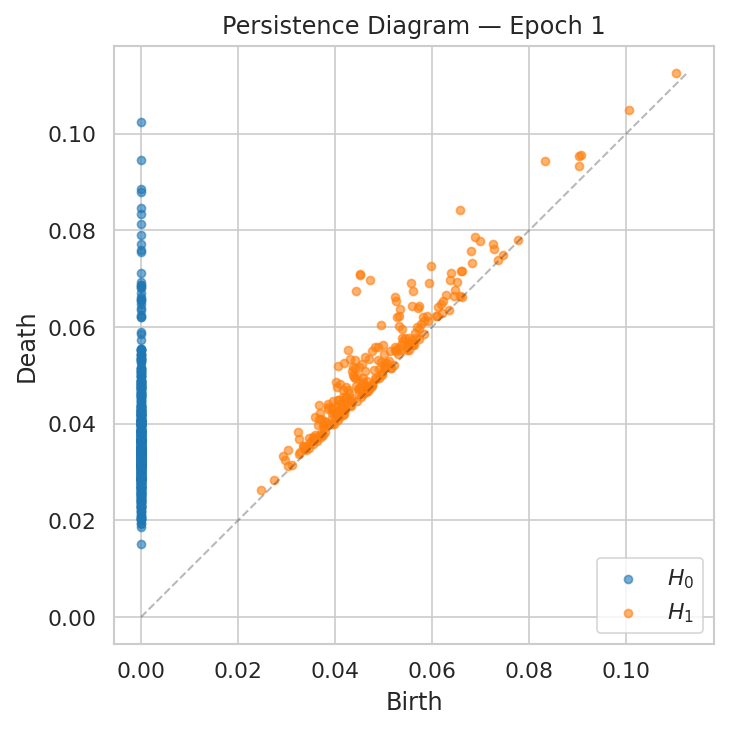
\includegraphics[width=\textwidth]{fashion_mnist_persistence_first.png}
    \caption{Epoch 1}
    \label{fig:persistence_first}
  \end{subfigure}
  \hfill
  \begin{subfigure}[t]{0.32\textwidth}
    \centering
    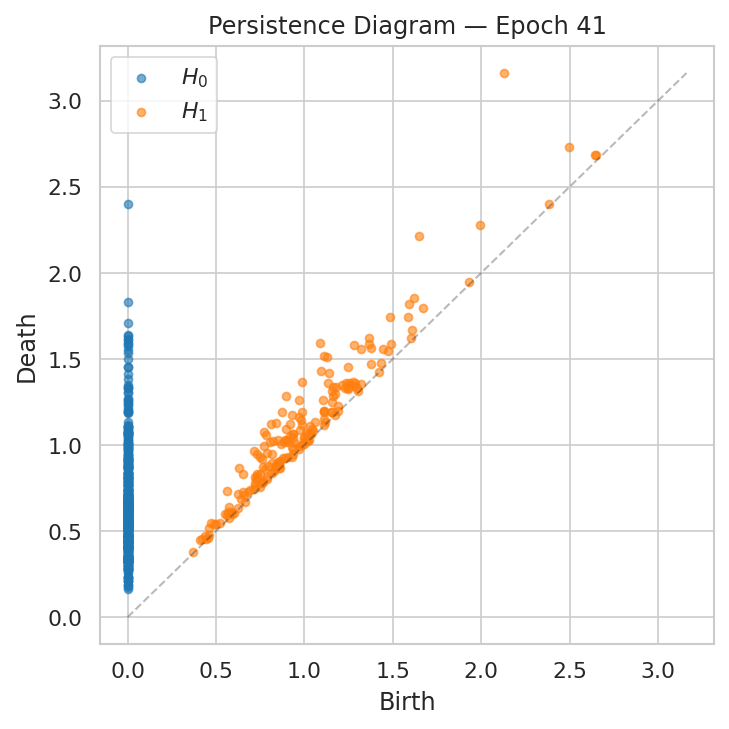
\includegraphics[width=\textwidth]{fashion_mnist_persistence_mid.png}
    \caption{Epoch 41}
    \label{fig:persistence_mid}
  \end{subfigure}
  \hfill
  \begin{subfigure}[t]{0.32\textwidth}
    \centering
    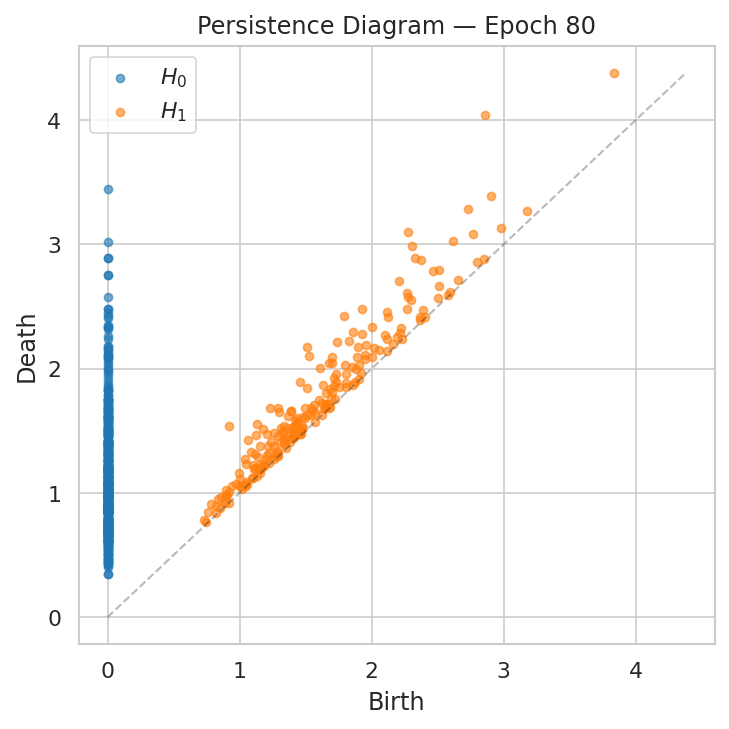
\includegraphics[width=\textwidth]{fashion_mnist_persistence_last.png}
    \caption{Epoch 80}
    \label{fig:persistence_last}
  \end{subfigure}
  \caption{Persistence diagrams of the bottleneck at epochs 1, 41, and 80
  (reference configuration: F-MNIST / CNN Shallow / $n=500$).}
  \label{fig:persistence_all}
\end{figure}

% -------------------------------------------------------------------------
\subsection{Interpretation}
\label{subsec:interpretation}

The results in \cref{tab:detection} show that topological detectors (TDA-D)
achieve a $100\%$ detection rate on all 8 tested configurations, with a
detection epoch significantly earlier than early stopping and comparable to
or earlier than loss gap. However, it would be premature to conclude that
topological invariants detect overfitting itself rather than a regime
change in representation dynamics that correlates with overfitting.

The three-phase pattern (compression $\to$ stabilization $\to$ fragmentation)
is consistent with results from Naitzat et al.~\cite{naitzat2020topologydeepneuralnetworks}
showing that successive layers simplify topology. Our contribution reveals
that this temporal simplification (across epochs) is not monotonic:
it partially reverses when the network begins to memorize.

Between epochs 40 and 80, the persistence diagrams in \cref{fig:persistence_all}
confirm this evolution: $H_1$ points (orange) progressively spread further
from the diagonal, signaling the creation of new loops in the activation
space that coincide with the acceleration of the train-val gap.

The rise in $\betti_1$ suggests that the network creates ``protrusions'' in
the representation space to isolate memorized examples, generating spurious
cyclic structures. This interpretation is consistent with work by Guss and
Salakhutdinov~\cite{guss2018characterizingcapacityneuralnetworks} and Ramamurthy et
al.~\cite{ramamurthy2018topologicaldataanalysisdecision}.

% =========================================================================
\section{Discussion}
\label{sec:discussion}

% -------------------------------------------------------------------------
\subsection{Comparison with Existing Approaches}
\label{subsec:comparaison}

The classical baselines fall into two categories. On one hand, weight norm and
loss gap trigger early but lack specificity: the former reflects optimizer
dynamics rather than overfitting, while the latter exhibits high variance
($\sigma$ up to $21.4$ epochs) that limits its reliability as an automatic
criterion. On the other hand, early stopping is highly specific but too
conservative: it requires val\_loss to stagnate for 10~consecutive epochs,
a condition that is rarely met in our setting (35\% detection rate).

TDA-based detectors occupy a middle ground. TDA-D achieves a 100\% detection
rate with moderate variance, offering a signal that classical methods do not
provide: a characterization of the geometry of internal representations,
rather than scalar training statistics. This geometric perspective makes the
detection complementary to, rather than redundant with, loss-based criteria.
TDA-CUSUM is generally later but potentially more robust to local fluctuations
in the topological time series.

% -------------------------------------------------------------------------
\subsection{Limitations}
\label{subsec:limitations}

We identify several important limitations:

\begin{enumerate}
  \item MLP case. TDA detectors are later than early stopping on
  MLP ($42.2$ vs.\ $34.6$). This can be explained by the fact that MLPs
  overfit differently (no weight sharing), producing a less structured
  topological evolution. This result shows that the topological signal is
  not universally early.

  \item Computational complexity. Vietoris-Rips computation in
  $\mathcal{O}(N^3)$~\cite{Edelsbrunner2009ComputationalTA} imposes
  $N \leqslant 500$--$1000$ points, which constitutes severe subsampling
  for large datasets.

  \item Layer choice. Only the bottleneck is analyzed. Other layers
  could present different or complementary signals.

  \item Threshold calibration. CUSUM thresholds and smoothed
  derivative parameters (window size, warm-up period) are fixed a priori.
  An automatic calibration procedure would strengthen the method.

  \item Experiment scale. Our architectures remain modest
  ($< 10^5$ parameters). Behavior on modern deep architectures (ResNets,
  Transformers) remains to be studied.

  \item Potential non-specificity. On CNN configurations, TDA-D
  triggers around epochs 19--28 while the validation loss minimum
  occurs much later (epochs 64--80), meaning that the topological
  transition precedes actual generalization degradation by 40--60 epochs.
  The detected signal may therefore reflect a learning regime change
  without direct causal link to overfitting. Experiments with
  regularization (dropout, weight decay) would verify whether the signal
  disappears when overfitting is prevented.
\end{enumerate}

% -------------------------------------------------------------------------
\subsection{Perspectives}
\label{subsec:perspectives}

\begin{itemize}
  \item Integration of TDA signal into an adaptive early stopping criterion,
  combining $\PE(H_1)$ and val\_loss, in order to benefit from both the
  earliness of the topological signal and the specificity of validation loss.
  \item Topological regularization: add a term penalizing the rise of
  $\betti_1$ in the loss function, in the spirit of neural
  persistence~\cite{rieck2019neural}, so as to actively prevent the
  fragmentation phase rather than merely detect it.
  \item Extension to modern architectures (ResNet, Vision Transformer) and
  large-scale data (ImageNet), requiring persistent homology approximations
  (sparse filtrations, landmarks), to assess whether the three-phase pattern
  generalizes beyond the small-scale architectures studied here.
  \item Study of higher-dimensional homology ($H_2$) to detect potential
  cavities in representations.
\end{itemize}

% =========================================================================
\section{Conclusion}
\label{sec:conclusion}

We conducted a systematic study of persistent homology of deep neural network
activations as a tool for early detection of overfitting. Across 8 experimental
configurations generated by a one-factor-at-a-time design over 3 datasets, 3 architectures, and 4 training sizes---with 5 independent runs each, we showed that:

\begin{enumerate}
  \item Topological invariants ($\betti_1$, $\PE(H_1)$) follow a three-phase
  pattern---compression, stabilization, fragmentation---reproducible across
  all tested CNN configurations.

  \item Detectors based on the smoothed derivative of $\PE(H_1)$ and $\betti_1$
  achieve a $100\%$ detection rate on all 8 configurations, triggering at
  epochs 18--28 on CNN architectures---30 to 55 epochs before early stopping
  when it fires (35\% of runs only).

  \item Invariant stability with respect to subsampling is comparable to
  inter-run variability (bootstrap ratio $\approx 1$).

  \item The topological signal is however not universally early: it is later
  on MLP, calling for caution regarding generalization.
\end{enumerate}

These results constitute an encouraging but not definitive proof of concept.
Extension to larger-scale architectures and tasks, as well as verification of
signal specificity (disappearance under regularization), are necessary
steps before claiming that TDA offers a significant practical advantage for
overfitting detection.

% =========================================================================
\printbibliography

\end{document}
